\documentclass[aspectratio=169,10pt]{beamer}
\usetheme{Madrid}
\usepackage{graphicx}
\usepackage{amssymb}

% Vô hiệu hóa shadow tránh lỗi vệt đen
\setbeamertemplate{blocks}[rounded][shadow=false]
\setbeamertemplate{navigation symbols}{}

% Color configuration
\definecolor{primaryblue}{RGB}{20, 55, 110}
\setbeamercolor{palette primary}{bg=primaryblue,fg=white}
\setbeamercolor{structure}{fg=primaryblue}

\begin{document}

% =========================================================================
% SLIDE 1: DEFINITION & GEOMETRIC MEANING
% =========================================================================
\begin{frame}{Graph of a Two-Variable Function: Definition}
    \begin{columns}[T]
        \begin{column}{0.56\textwidth}
            \begin{block}{Definition (Graph in $\mathbb{R}^3$)}
                \small
                The \textbf{graph} of a function of two variables $f$ with domain $D$ is the set of all points $(x, y, z) \in \mathbb{R}^3$ such that $z = f(x, y)$ and $(x, y) \in D$:
                \[
                    \mathrm{Graph}(f) = \{(x, y, z) \in \mathbb{R}^3 \mid z = f(x, y), \, (x, y) \in D\}.
                \]
            \end{block}

            \vspace{0.1cm}

            \begin{block}{Geometric Transition ($2\mathrm{D} \to 3\mathrm{D}$)}
                \small
                \begin{itemize}
                    \item In single-variable calculus, the graph of $y = f(x)$ is a \textbf{curve} in $\mathbb{R}^2$.
                    \item In multivariable calculus, the graph of $z = f(x, y)$ is a \textbf{surface} $S$ in $\mathbb{R}^3$.
                \end{itemize}
            \end{block}
        \end{column}

        \begin{column}{0.42\textwidth}
            \centering
            \vspace{0.15cm}
            
\includegraphics[width=0.92\linewidth, keepaspectratio]{CurveToSurfaceScene.png}
            \vspace{0.1cm}
            {\tiny \textcolor{gray}{\textit{From 2D curves to 3D surfaces}}}
        \end{column}
    \end{columns}
\end{frame}

% =========================================================================
% SLIDE 2: VERTICAL LINE TEST
% =========================================================================
\begin{frame}{The Vertical Line Test in $\mathbb{R}^3$}
    \begin{columns}[T]
        \begin{column}{0.56\textwidth}
            \begin{block}{The Vertical Line Criterion}
                \small
                A surface $S \subset \mathbb{R}^3$ represents the graph of a single-valued function $z = f(x,y)$ if and only if:
                \begin{itemize}
                    \item Every \textbf{vertical line} through $(x_0, y_0) \in D$ (parallel to the $z$-axis) intersects the surface $S$ at \textbf{exactly one point}:
                    \[
                        P = (x_0, y_0, f(x_0, y_0)).
                    \]
                    \item If a vertical line intersects the surface at more than one point, the surface \textbf{cannot} be expressed as a single function $z = f(x,y)$.
                \end{itemize}
            \end{block}
        \end{column}

        \begin{column}{0.42\textwidth}
            \centering
            \vspace{0.15cm}
            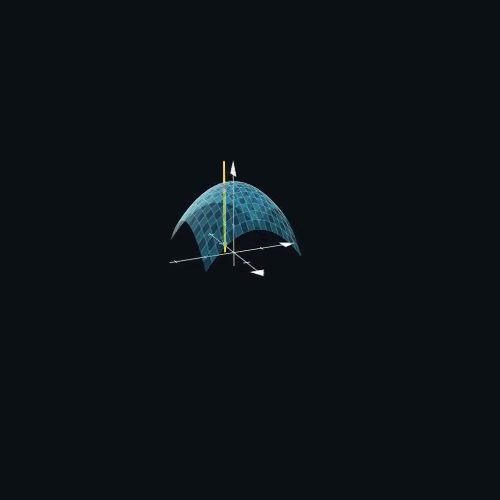
\includegraphics[width=0.92\linewidth, keepaspectratio]{VerticalLineTestScene.png}
            \vspace{0.1cm}
            {\tiny \textcolor{gray}{\textit{Single intersection $(x_0, y_0, z_0)$ per vertical line}}}
        \end{column}
    \end{columns}
\end{frame}

% =========================================================================
% SLIDE 3: FUNDAMENTAL SURFACE FAMILIES
% =========================================================================
\begin{frame}{Fundamental Surface Families}
    \begin{columns}[T]
        \begin{column}{0.56\textwidth}
            \begin{block}{Standard Quadric \& Explicit Surfaces}
                \small
                \begin{itemize}
                    \item \textbf{Plane}: $z = ax + by + c$
                    \item \textbf{Circular Paraboloid}: $z = x^2 + y^2$
                    \item \textbf{Elliptic Paraboloid}: $z = \frac{x^2}{a^2} + \frac{y^2}{b^2}$
                    \item \textbf{Circular Cone}: $z = \sqrt{x^2 + y^2}$
                    \item \textbf{Upper Hemisphere}: $z = \sqrt{R^2 - x^2 - y^2}$
                    \item \textbf{Hyperbolic Paraboloid (Saddle)}: 
                    \[
                        z = x^2 - y^2
                    \]
                \end{itemize}
            \end{block}
        \end{column}

        \begin{column}{0.42\textwidth}
            \centering
            \vspace{0.15cm}
            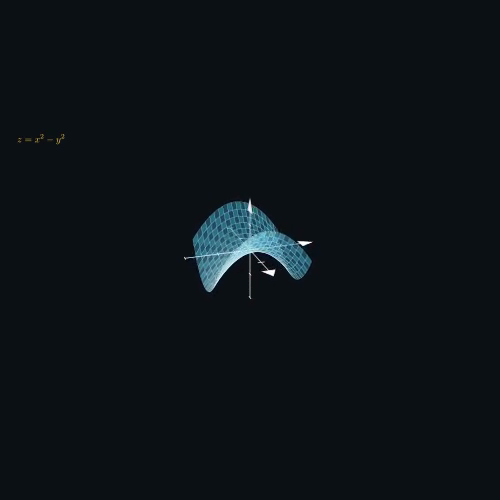
\includegraphics[width=0.92\linewidth, keepaspectratio]{SaddleSurfaceScene.png}
            \vspace{0.1cm}
            {\tiny \textcolor{gray}{\textit{Hyperbolic Paraboloid (Saddle Surface)}}}
        \end{column}
    \end{columns}
\end{frame}

\end{document}
